% define the type of document I want to make (article), set 12pt font and letter-sized paper
\documentclass[12pt, letterpaper]{article}
\usepackage[margin=1in]{geometry}
% the natbib package lets me use extra citation commands, authoryear sorts bibliography by author last name, then year of publication
\usepackage[authoryear]{natbib}
% the hyperref package lets me insert a hyperlink, and makes table of contents and references clickable
\usepackage{hyperref}
% graphicx allows....graphics
\usepackage{graphicx}
% letting LaTeX do line breaks easier so it doesn't complain about hboxes
\setlength{\emergencystretch}{5pt}

% enter the document environment to begin!
\begin{document}

% set the title
\title{Final Project - PHYS 5391}
% set author
\author{Elizabeth Vandegriff}
% set date as current date
\date{\today}

% make the above title/author/date visible
\maketitle
% leave the rest of the title page blank
\newpage
% create a table of contents based on the sections I define throughout the doc
\tableofcontents
% start sections on new page after table of contents
\newpage

\section{Intro} \label{intro}

In space physics, the Auroral Electrojet (AE) provides a measure of the magnetic activity in the auroral region, calculated by subtracting the maximum and minimum of the North magnetic field components of about 12 auroral zone observatories between latitudes of 65 and 70 degrees. Space weather models can produce the same AE index using the output of their model, with varying success. In the Space Weather Modeling Framework (SWMF), the simulated Auroral Electrojet (AE) index is not always a useful numeric because of how approximately it is currently calculated. Unlike the real-life AE calculation, the SWMF calculates AE using 24 virtual magnetometer stations at a fixed 70 degrees.

This final project provides an alternative and more realistic model AE calculation using the SWMF model output. The end result is a set of values for AE over a period of serveral days (September 6-8, 2017) that minimizes both the root-mean-square error (RMSE) and the number of virtual magnetometers used in the calculation.

Section \ref{calc} describes the setup and code involved in calculating the auroral indices. Section \ref{vis} shows a visual representation of the calculated data, draws conclusions from the data visualization, and provides details of the optimization process. Finally, Section \ref{conc} concludes and suggests future ideas for the project.


\section{AE Calculation} \label{calc}

To calculate AE from simulation output, it is necessary to first describe the conditions of the model that produced this output. The Space Weather Modeling Framework is highly customizable, and takes inputs such as solar wind conditions to attempt to reproduce observed events. Output for such a run produces thousands of files that describe the conditions around Earth during a specified time range. Among these are a set of files containing magnetometer readings for virtual ground magnetometers at various latitudes and longitudes.

In this project, the magnetic field values from these magnetometer files will be used to calculate AE. For the run analyzed in this project, the SWMF output provides magnetometers on a one-degree by one-degree grid, for latitudes from 0 to 85 degrees, and longitudes from 0 to 360 degrees. In addition, this run has a 10-second frequency, meaning it creates files with new values for every 10 seconds of simulated time from September 6, 2017 18:00:00 to September 9, 2017 00:00:00.
AE will be calculated by restricting the array of northward magnetic field readings to only a specified latitude range (65 to 70 degrees), and subtracting the minimum and maximum values of the resulting array. The python script \texttt{calc\_ae.py} performs the AE calculation for each file (aka each 10-second timestep), saves the AE value into a dictionary, and writes the dictionary into a python pickle.

Without any modifications, \texttt{calc\_ae.py} calculates AE using the full resolution of the output - that is, taking the max and min of all magnetometers from 0 to 360 degrees longitude for each latitude. Because another goal of the project is to reproduce AE using the least possible number of magnetometers, another step is added to specify how many magnetometers should be used in the AE calculation. This can be implemented using \texttt{scipy.signal.resample} in Python, which resamples an array at a specified rate. This enables the user to run \texttt{calc\_ae.py} using a decreased number of magnetometers.

Below are the steps to calculate AE for a single magnetometer file:
\begin{itemize}
  \item Open the magnetometer file using SpacePy
  \item Access the northward magnetic field readings array which contains values for all virtual magnetometers
  \item Select portion of array that corresponds to 65-70 degrees latitude
  \item Resample the array to use specified number of magnetometers per degree latitude
  \item Calculate min and max of array
  \item AE is the subtraction of the min and the max
  \item (Extra step: calculate the \textit{total} number of magnetometers used to calculate AE by multiplying the number of magnetometers used per degree latitude by the number of degrees covered by the latitude range. For this analysis, the latitude range is 6 degrees, so the number of magnetometers used per degree is multiplied by 6)
\end{itemize}

Calculated indices were verified by hand for several cases to ensure that they were correct. Python script \texttt{calc\_ae.py} loops through the specified files and calculates an AE for each timestep. Because of the 10-second frequency, there are almost 20,000 magnetometer files in the entire run. While all of these files are used in the AE calculation, it would take too long to process all files each time the code is run during the development, testing, and debugging processes. To work around this, the code is written to toggle between the full version (processing all magnetometer files) and a debugging version (processing only a few selected files). As well as restricting the number of files, the debugging version prints additional information to the screen for verification purposes.

The goal of calculating AE using SWMF model output has been achieved, and the new goal is to determine the minimum number of magnetometers that are needed to reproduce a satisfactory AE.

The first step of this process is to run \texttt{calc\_ae.py} for a decreasing number of magnetometers. The Python script \texttt{create\_range\_pkls.py} is a short script that allows the user to specify a start, stop, and step range, then loops through and runs \texttt{calc\_ae.py} for each step size (aka number of magnetometers).


\section{AE Data Visualization and Analysis} \label{vis}

The next step toward determining the minimum number of magnetometers needed for the AE calculation is to visualize the AE data and compare the calculations done using different numbers of magnetometers.

Running \texttt{create\_range\_pkls.py} with a start of 10, stop of 361, and step of 10 yields 36 calculations of AE over the period of the simulation, using a decreasing number of magnetometers.

Plotting AE calculated using all the magnetometer stations (Fig. (\ref{fig:360})) shows the ideal AE output of the model.

\begin{figure}[!ht]
  \centering
  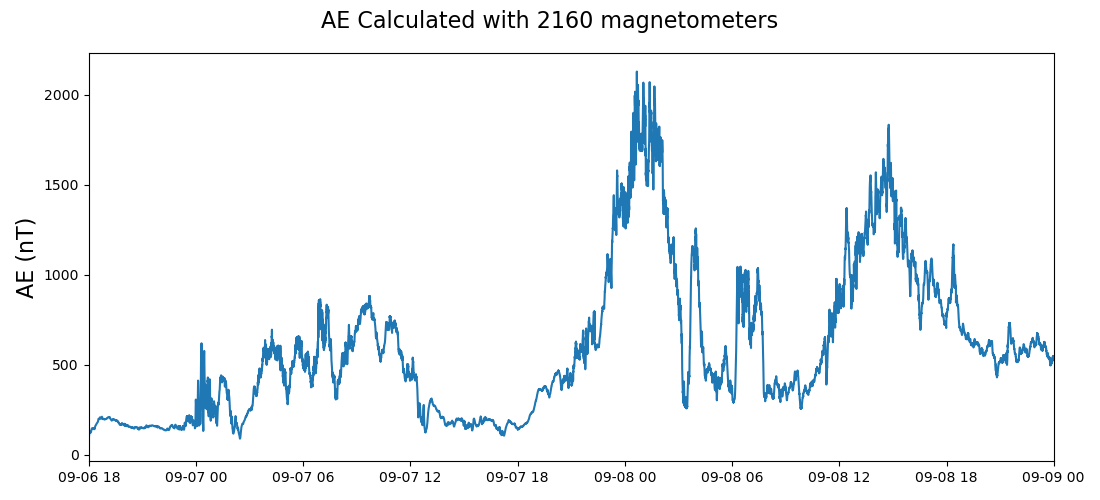
\includegraphics[width=14cm]{../ae_plots_LaTeX/ae_2160.png}
  \caption{AE calculated from simulation output using all 2160 magnetometers.}
  \label{fig:360}
\end{figure}

Overplotting AE curves calculated using fewer and fewer magnetometer stations becomes unhelpful the more curves are added. Plotting an AE curve for each pickle created from \texttt{create\_range\_pkls.py} results in a severaly overloaded plot, shown in Figure (\ref{fig:allae}). This plot does not give a quantitative or ever qualitative picture of how magnetometer number affects the AE calculation.

\begin{figure}[!ht]
  \centering
  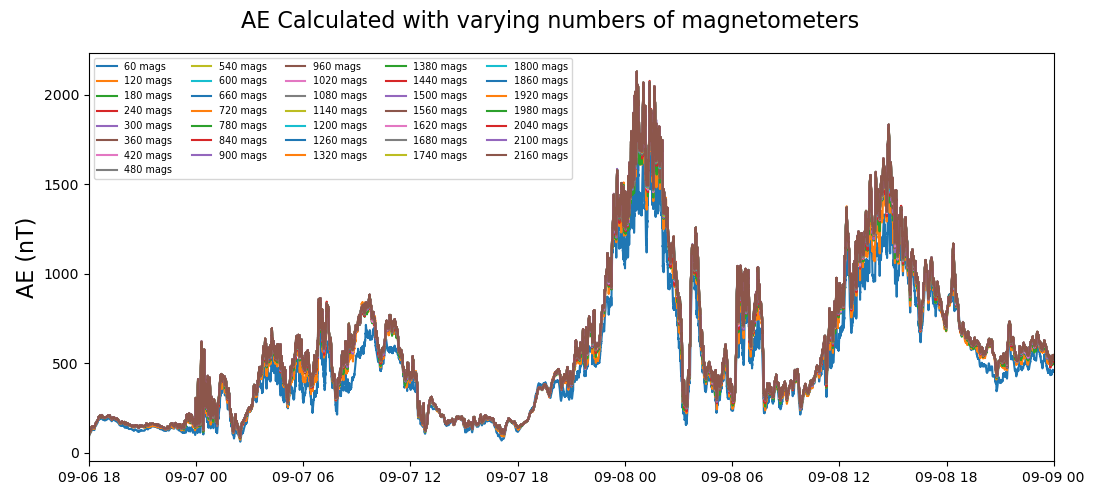
\includegraphics[width=14cm]{../ae_plots_LaTeX/all_ae.png}
  \caption{AE calculated from simulation output using a range of magnetometers.}
  \label{fig:allae}
\end{figure}

Another possible technique would be to plot each curve successively, saving a copy of the figure each time a new curve is added. The animated gif included in the git submission shows a progression of the AE curves being plotted atop each other, starting with the lowest magnetometer curve. In the gif, there is some indication that very low magnetometer numbers give a visually different curve from AE calculated with all the magnetometers, but there is still nothing quantitative to say about the relationship.

A better way to compare the different curves is to set AE calculated with all magnetometers as the idea AE, and compare it to other AE curves using root-mean-square error. Figure (\ref{fig:rmse}) shows the RMSE as a function of the number of magnetometers used to calculate AE.

\begin{figure}[!ht]
  \centering
  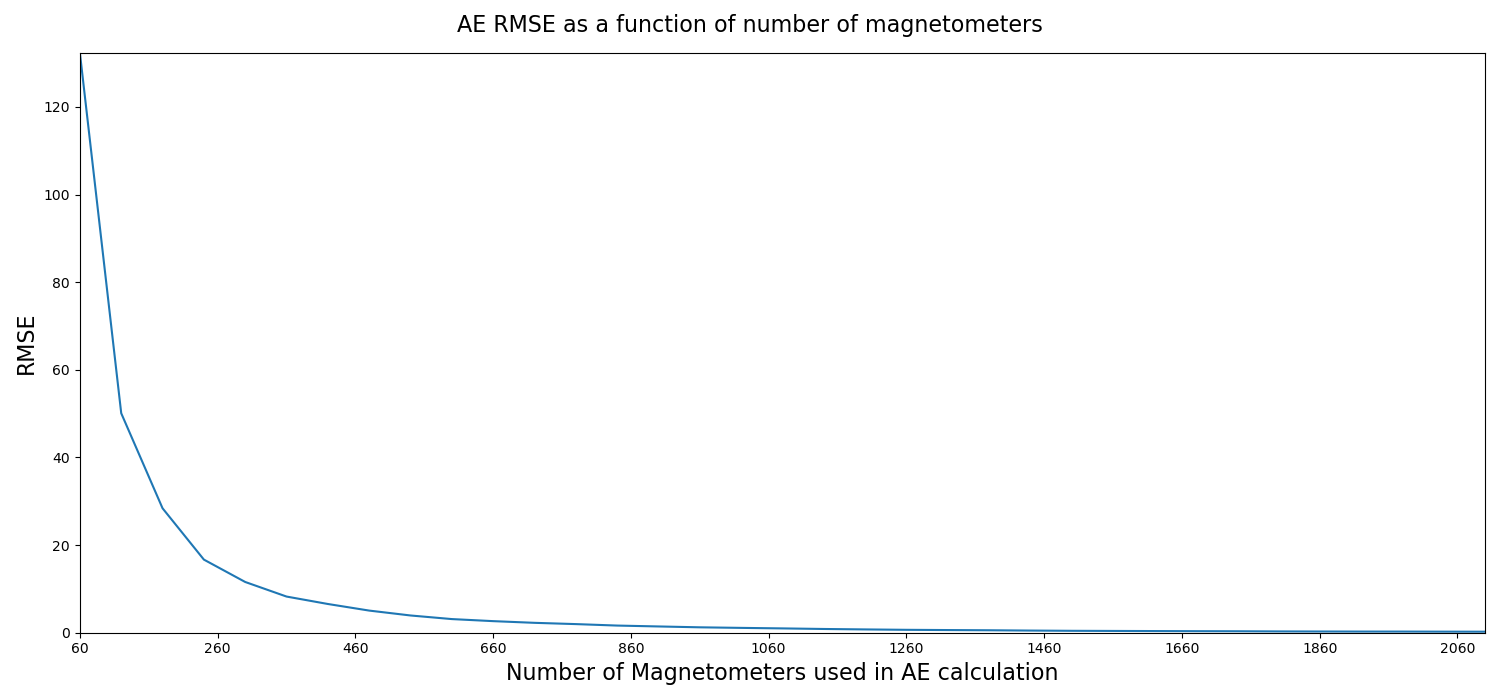
\includegraphics[width=14cm]{../ae_plots_LaTeX/rmse_v_num_mags.png}
  \caption{RMSE between AE curves as a function of the number of magnetometer stations used in the calculation.}
  \label{fig:rmse}
\end{figure}


Clearly there is a sharp decline in RMSE as more magnetometers are used in the calculation. But where is the knee point of this curve? That is, what number of magnetomters that minimizes both itself and RMSE? One possible answer to this question lies in a python package called ``kneed'', which computes the knee point of a curve. Using this package to calculate and plot the knee point of the RMSE curve yields Figure (\ref{fig:rmseKnee}).

\begin{figure}[!ht]
  \centering
  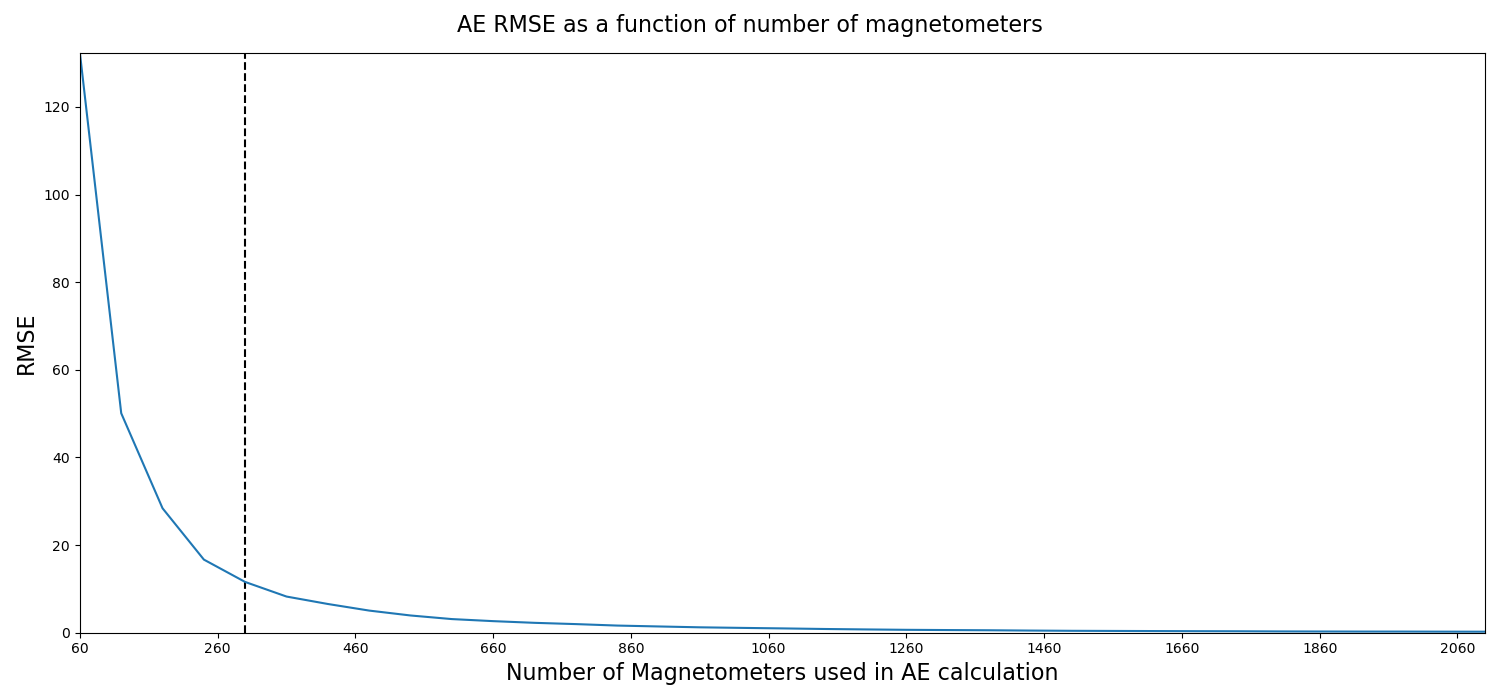
\includegraphics[width=14cm]{../ae_plots_LaTeX/rmse_v_num_mags_vline.png}
  \caption{RMSE between AE curves shown with optimized knee point at 300 magnetometers.}
  \label{fig:rmseKnee}
\end{figure}

Thus, the optimized number of magnetometer stations to use for the AE calculation is 300, or 50 per degree latitude. AE for 300 magnetometers is shown in Figure (\ref{fig:ae300})

\begin{figure}[!ht]
  \centering
  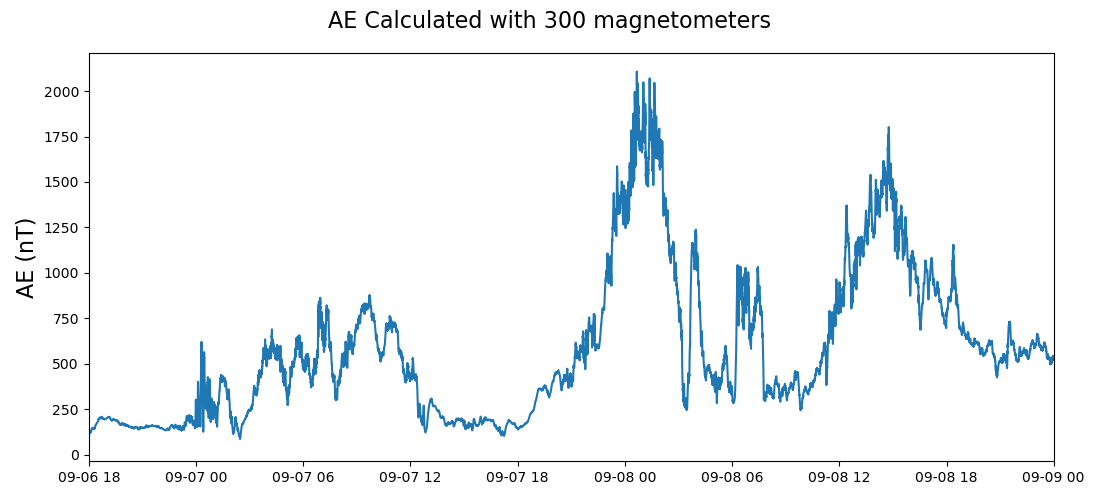
\includegraphics[width=14cm]{../ae_plots_LaTeX/ae_300.png}
  \caption{AE calculated from simulation output using an optimized 300 magnetometers.}
  \label{fig:ae300}
\end{figure}

Although the focus of this project is AE, the scripts in this project calculate AL and AU as well, which can be plotted together as in Figure (\ref{fig:alau300})

\begin{figure}[!ht]
  \centering
  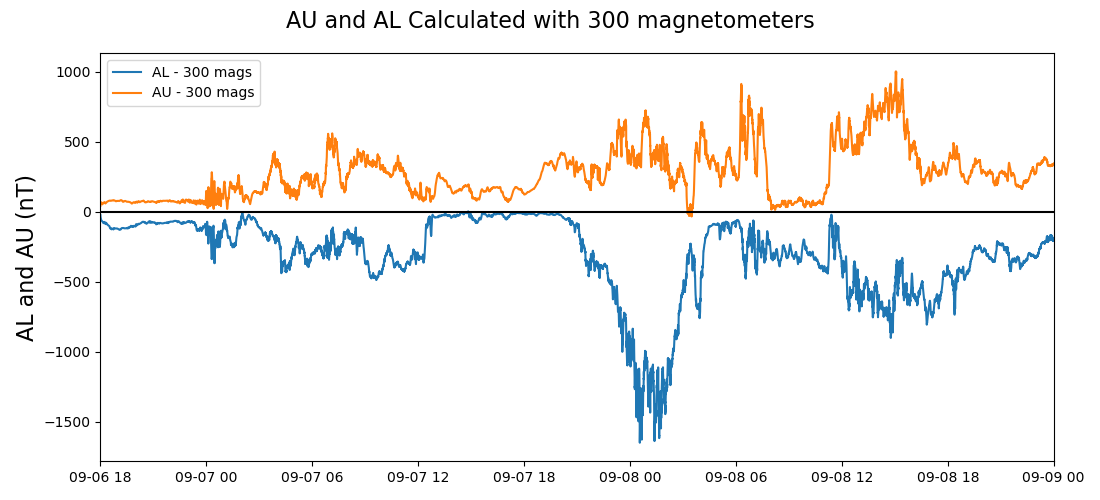
\includegraphics[width=14cm]{../ae_plots_LaTeX/al_au_300.png}
  \caption{AL and AU calculated from simulation output using an optimized 300 magnetometers.}
  \label{fig:alau300}
\end{figure}

\section{Conclusions} \label{conc}

Overall, this project was a success, and reached the goals of calculating and optimizing AE based on Space Weather Modeling Framework output. The process required Python scripting, file I/O in Python, and data visualization in Python, as well as general use of good coding habits, critical thinking, and creativity.

Although the goals of the project have been achieved, there is much future work to consider for this AE calculation project. First, while finding the knee point may prove to be helpful, using more stations to get a more accurate AE may prove advantageous if the number of magnetometers used does not significantly affect the calculation's run time. Second, comparing the AE calculated in this project to the AE that the SWMF currently calculates will be a measure of how beneficial the improved AE calculation is. Third, performing analyses of AL, AU, and Ao may be of use in determining the project's effectiveness. Finally, comparing the model AE data to the AE data calculated from real magnetometer stations will show how successful the model itself is, and if the AE calculation done in this project is sufficient for comparison. 




\end{document}
